\documentclass[11pt]{article}
\usepackage{mathtools}
\usepackage{mdframed}
\usepackage{fullpage}
\usepackage{amsfonts}
\usepackage{tikz}
\usepackage{fancyhdr}
\usepackage{lastpage}
\usetikzlibrary{automata, positioning}


%edit this for each class
\newcommand\name{John Collin Vincent}
\newcommand\classname{Com S 311}
\newcommand\assignment{Homework 6}


\newcounter{excounter}
\setcounter{excounter}{1}
\newcommand\ques[2]{\vskip 1em  \noindent\textbf{\arabic{excounter}\addtocounter{excounter}{1}.} \emph{#1} \noindent#2}
\newenvironment{question}{\ques{}\begin{quote}}{\end{quote}}
\newenvironment{subquestion}[1]{#1) \begin{quote}}{\end{quote}}

\pagestyle{fancy}
\rfoot{\name, page \thepage/\pageref{LastPage}}
\cfoot{}
\rhead{}
\lhead{}
\renewcommand{\headrulewidth}{0pt}
\renewcommand{\footrulewidth}{0pt}
\DeclarePairedDelimiter\ceil{\lceil}{\rceil}
\DeclarePairedDelimiter\floor{\lfloor}{\rfloor}


\begin{document}


  {\bf \classname \hspace{1cm} \assignment\hfill \name}
  \vskip 2em


  \begin{question}
    \begin{subquestion}{a}
      \centering
      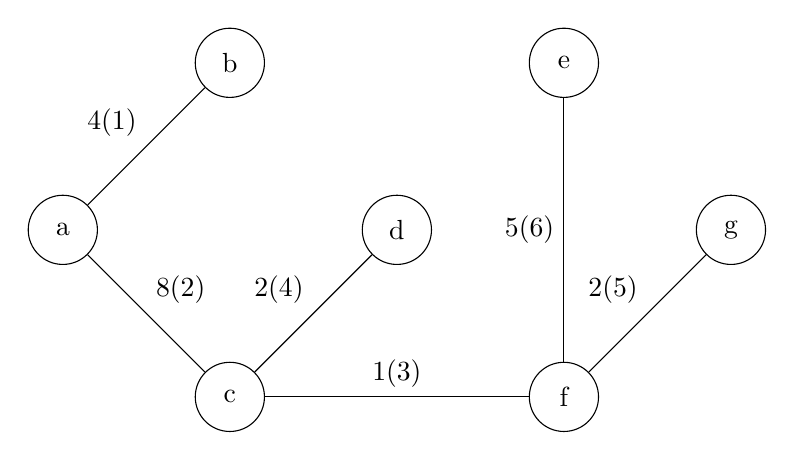
\begin{tikzpicture}[node distance=3cm,bend angle=45,auto]
        \node[state] (n1) {a};
        \node[state] (n2) [above right of = n1] {b};
        \node[state] (n3) [below right of = n1] {c};
        \node[state] (n4) [below right of = n2] {d};
        \node[state] (n5) [above right of = n4] {e};
        \node[state] (n6) [below right of = n4] {f};
        \node[state] (n7) [above right of = n6] {g};

        \path[-] (n1)
          edge node {$4(1)$} (n2)
          edge node {$8(2)$} (n3);

        \path[-] (n3)
          edge node {$2(4)$} (n4)
          edge node {$1(3)$} (n6);

        \path[-] (n6)
          edge node {$2(5)$} (n7)
          edge node {$5(6)$} (n5);
      \end{tikzpicture}
    \end{subquestion}

    \begin{subquestion}{b}
      \centering
      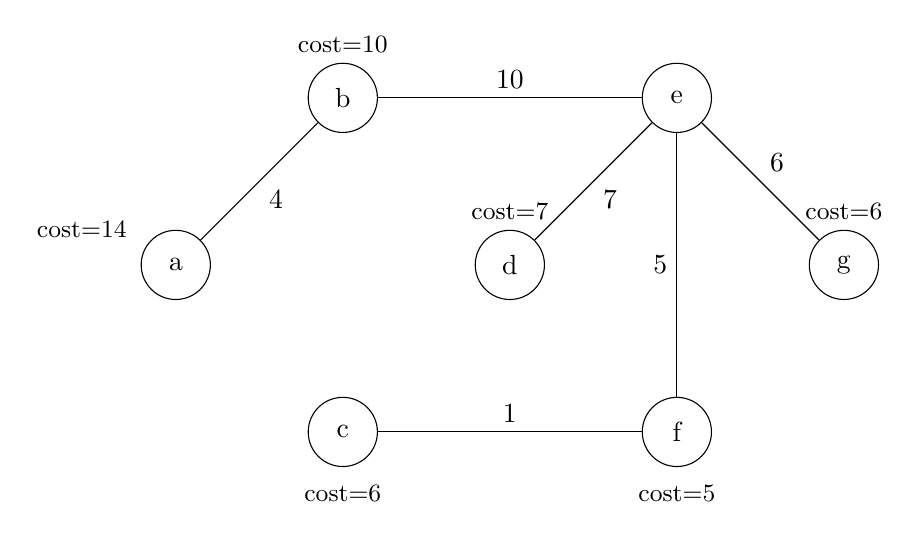
\begin{tikzpicture}[node distance=3cm,bend angle=45,auto]
        \node[state, label={[left = .5cm]\small cost=14}] (n1) {a};
        \node[state, label={[above]\small cost=10}] (n2) [above right of = n1] {b};
        \node[state, label={[below = 1cm]\small cost=6}] (n3) [below right of = n1] {c};
        \node[state, label={[above]\small cost=7}] (n4) [below right of = n2] {d};
        \node[state] (n5) [above right of = n4] {e};
        \node[state,label={[below = 1cm]\small cost=5}] (n6) [below right of = n4] {f};
        \node[state,label={[above]\small cost=6}] (n7) [above right of = n6] {g};

        \path[-] (n3)
          edge node {$1$} (n6);

        \path[-] (n2)
          edge node {$10$} (n5)
          edge node {$4$} (n1);

        \path[-] (n5)
          edge node {$7$} (n4)
          edge node {$6$} (n7);

        \path[-] (n6)
          edge node {$5$} (n5);
      \end{tikzpicture}
    \end{subquestion}
  \end{question}
  \clearpage
  \begin{question}
    Assume there is a graph $G$ such that the graph resulting from running this algorithm $G'$ is
    not a MST of $G$. $G'$ prime cannot have any cycles since if there is a cycle in $G'$ the largest edge in the cycle will be removed before the algrorithm finishes, since it can be removed without leaving any disconnected components. This means that $G'$ is at least a spanning
    tree of $G$. if $G'$ is not a minimum spanning tree that means there must be a edge $e$ in $G'$
    that can be removed and replaced with a path $p$ in $G$ that connects the two components
    connected by $e$, and the sum of the weights in $|p| < |e|$. This can't be the case though
    because if it was $e$ would have been removed from $G'$ before any of the edges in $p$ were visited, since removing $e$ would still keep the components connected through $p$ and
    $e$ must have a weight larger than every edge in $p$. This contradicts $G'$ not being a MST of
    $G$ and proves that this algorithm results in a MST of $G$
  \end{question}

  \begin{question}
  \end{question}

\end{document}
